\documentclass[xcolor=svgnames]{beamer}
\usetheme{Singapore}
\setbeamertemplate{footline}[frame number]
\setbeamertemplate{navigation symbols}{}
\setbeamertemplate{itemize item}[triangle]
\setbeamertemplate{itemize subitem}[ball]


\usepackage{contour}


%\usefonttheme{serif}
%\usepackage{fontspec}
%\setmainfont{Linux Libertine O}

\usepackage{tikz}
\usetikzlibrary{arrows,shapes,positioning,calc, shapes.geometric,shapes.arrows}


\usepackage[group-separator={,},group-minimum-digits={3}]{siunitx}


\usepackage{makecell}
\usepackage{caption}
\usepackage{subcaption}
\usepackage{graphicx}

\title{Identification of Functional Implementation in Conventional Applications and Transformation to Smart Contracts}
\author{Qiqi Gu\\P0907870}
\institute{%
\tikz[baseline, inner sep=0pt, remember picture]{\node [anchor=base, baseline, inner sep=0pt, align=center] (mpi text)
	{Faculty of Applied Sciences\\Macao Polytechnic University, Macao SAR, China};
}%
}
\date{March 2, 2022}

\parskip=20pt

\begin{document}
\newcommand{\etal}[1]{#1~{\it et al.}}

%\tikzset{every picture/.style={/utils/exec={\sffamily}}}

\tikzset{Process/.style={rectangle, draw=black, inner sep=0.1cm, text centered, align=center}}
\tikzset{Arrow/.style={thick, ->, >=stealth}}

{
\usebackgroundtemplate{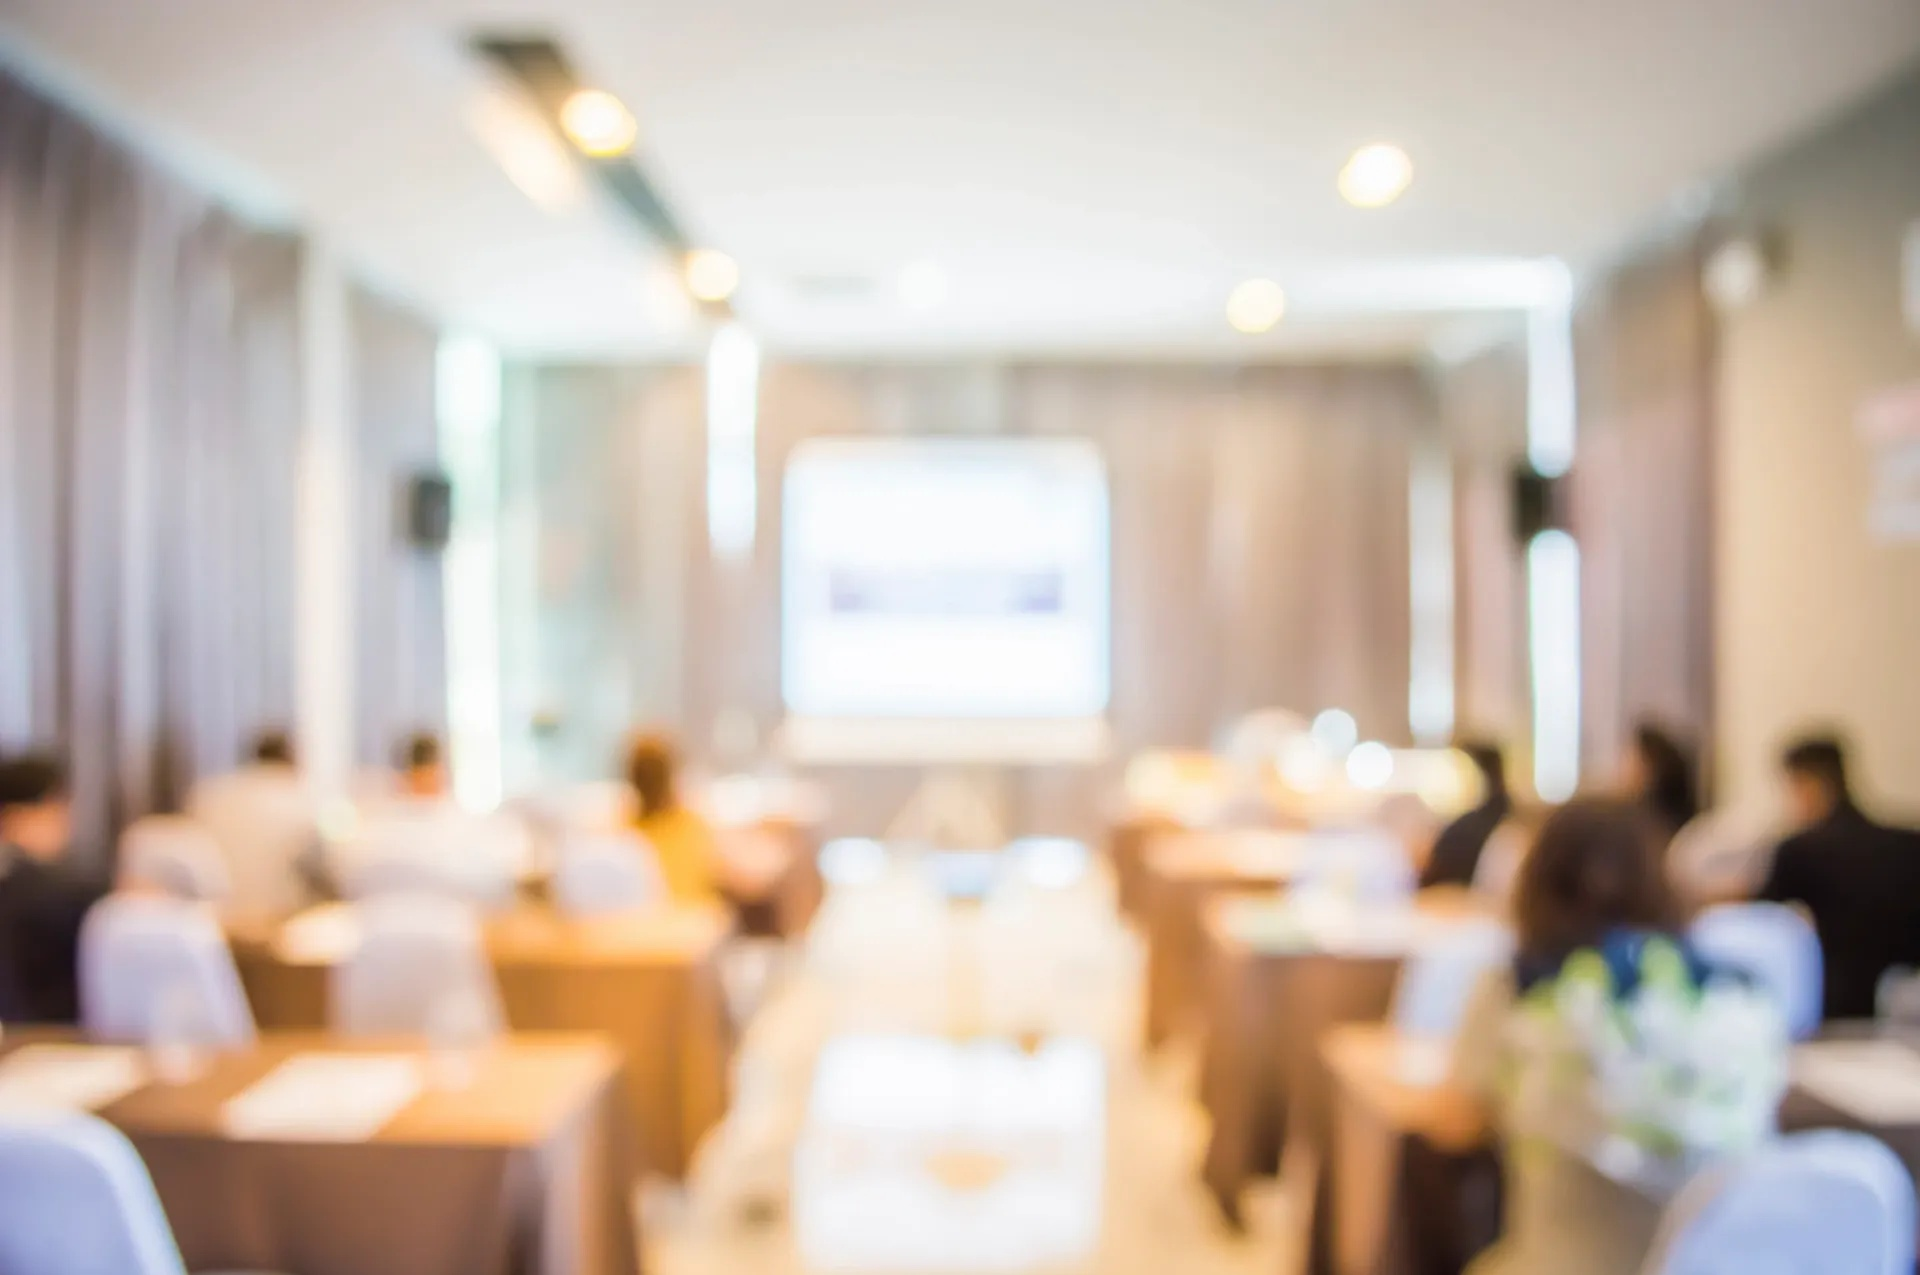
\includegraphics[height=\paperheight]{background.jpg}}%

\begin{frame}[plain]
	\maketitle

	\begin{tikzpicture}[overlay, remember picture]
	\node[inner sep=0pt, left=0.2cm of mpi text]{
\includegraphics[width=1.2cm]{mpi-logo.png}};
	\end{tikzpicture}
\end{frame}
}

\begin{frame}{Outline}
	\tableofcontents
\end{frame}

\section{Introduction}
\begin{frame}{Smart Contracts}
\begin{itemize}
\item A smart contract is a program running on a blockchain platform.
\item Using smart contracts has many advantages, e.g., reduce the need of trust, reduce enforcement costs.
\item Businesses often use smart contracts as a signed contract or an agreement to regulate the stakeholders~[1].
\item<2-> It is difficult to implement smart contracts correctly from scratch~[32].
\end{itemize}
\end{frame}

\begin{frame}{Using Smart Contracts}

\begin{itemize}
\item Businesses already use conventional software to help deal with their business logic.
\item Some of these software are open source and hosted online.
\item We believe it is ideal to transform these applications into smart contracts.
\end{itemize}

\end{frame}

\begin{frame}[t]{Transformation}

\begin{figure}
\centering

\begin{tikzpicture}
\onslide<1,2>{
\node (req) [Process] {Requirement Documents};
\node (sc1) [Process, below=of req] {Smart Contract};
\draw [Arrow] (req) -- (sc1);
}

\onslide<1,3>{
\node (impl) [Process, right=of req, xshift=1.5cm] {Source Code};
\node (sc2) [Process, below=of impl] {Smart Contract};
\draw [Arrow] (impl) -- (sc2);
}
\end{tikzpicture}
\end{figure}

\only<2>{

\includegraphics[width=0.8em]{check.png} Requirement documents capture raw information.


\includegraphics[width=0.8em]{cross.png} Open source projects typically do not publish such documents.
}

\only<3>{

\includegraphics[width=0.8em]{check.png} Application source code are widely available.


\includegraphics[width=0.8em]{cross.png} The code may contain too many details and noises.
}

\end{frame}


\begin{frame}{Identification and Transformation}

\begin{enumerate}
\item identify which conventional applications are transformable

\item implement algorithms to transform these applications to smart contracts
\end{enumerate}
\end{frame}


\section{Background}
\begin{frame}[t]{Blockchain Platforms}
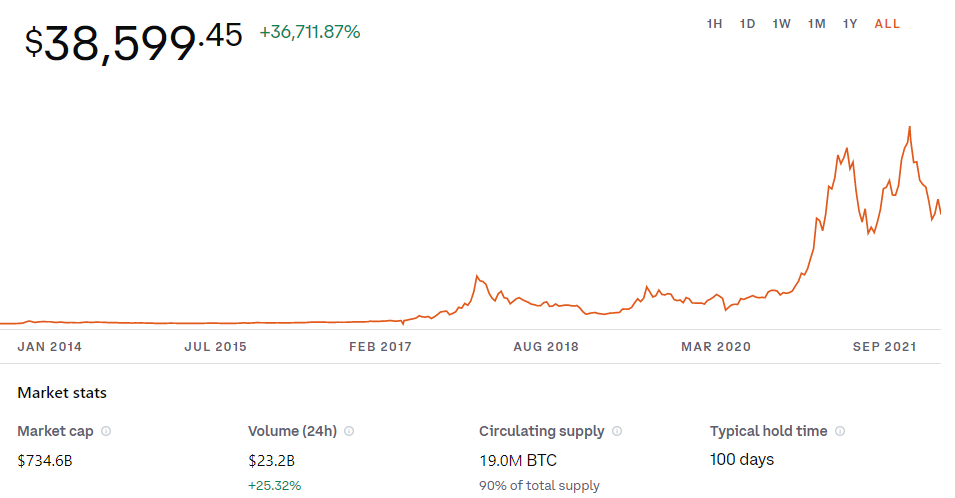
\includegraphics[width=0.9\linewidth]{bitcoin-price}

Market cap of BitCoin reached \$780 billion in January 2022.

The Taproot upgrade took place in November 2021 enabled Bitcoin to execute smart contracts in the core layer.
\end{frame}

\begin{frame}[t]{Blockchain Platforms}
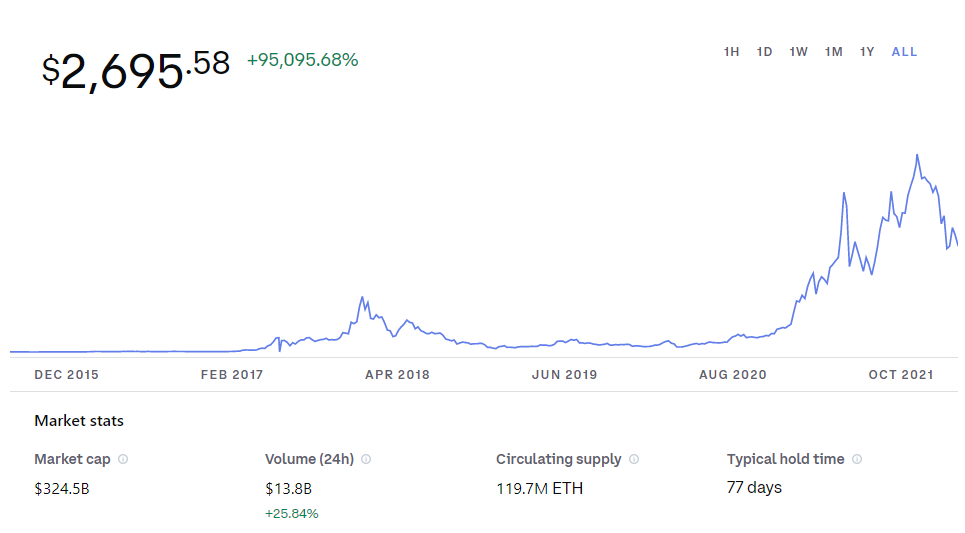
\includegraphics[width=0.9\linewidth]{ethereum-price}

Ethereum is the second largest blockchain platform with market cap of \$360 billion.

It has more mature support of smart contract.
\end{frame}


\begin{frame}{Permissioning of Blockchain Platforms}

\begin{table}
\small
%\setlength\tabcolsep{10pt}
\renewcommand*{\arraystretch}{2}
\begin{tabular}{ll}
Permissionless                                                              & Permissioned                                                \\ \hline
\makecell[l]{Everyone can view the transaction data, \\make transactions, or send queries.} & \makecell[l]{A central authority determines \\who can join the blockchain.} \\
Bitcoin, Ethereum                                                           & \onslide<2->{Hyperledger Fabric}                                          \\
\end{tabular}
\end{table}

\end{frame}

\begin{frame}
\frametitle{

\includegraphics[height=1cm]{hyperledgerfoundation_horizontal-dark.png}
\qquad
\onslide<2->{
\includegraphics[height=1.1cm]{Hyperledger_Fabric_Logo.png}}
}

\begin{itemize}
\item Hyperledger is an umbrella project of open source blockchains and related tools.
\begin{itemize}
\item started in December 2015 by the Linux Foundation
\item gets consistent contributions from IBM, Intel, and so on.
\end{itemize}

\item<2-> In Hyperledger, Fabric is the most developed platform.
\begin{itemize}
\item run smart contracts developed in Java, JavaScript, or NodeJS
\item preferred by businesses
\end{itemize}
\end{itemize}
\end{frame}


\begin{frame}[t]{Smart Contracts vs.\ DApp}

\begin{itemize}
\item DApp is short for decentralized application.
\begin{onlyenv}<1>
\begin{enumerate}
\item open source. There is no entity controlling the application. Its data are stored in a public blockchain.
\item has tokens to reward user participation. Users spend tokens to interact with the application.
\item be changed in response to consensus of its users~[3]
\end{enumerate}
\end{onlyenv}

\item<2-> Development of DApp

\begin{onlyenv}<2>
\begin{figure}
\centering
\begin{tikzpicture}[node distance=0.5cm and 1cm]
\node (whitepaper) [Process] {release whitepaper};
\node (program) [Process, below=of whitepaper] {release reference program \\for mining or interaction};
\node (mine) [Process, below=of program] {mine or stake};
\node (proposals) [Process, below=of mine] {write improvement proposals};


\node (whitepaper-icon) [left=of whitepaper] {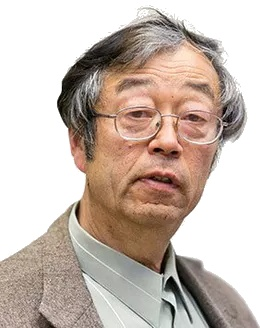
\includegraphics[width=0.5cm]{satoshi.jpg}};

\node (program-icon) [opacity=0.9] at (whitepaper-icon |- program) {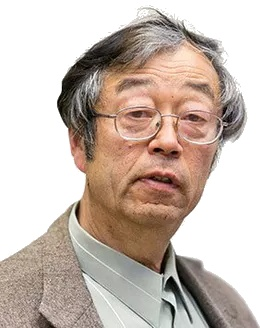
\includegraphics[width=0.5cm]{satoshi.jpg}};
\node                [opacity=0.1] at (whitepaper-icon |- program) {
\includegraphics[width=0.5cm]{worldwide.png}};

\node (mine-icon) [opacity=0.7] at (program-icon |- mine) {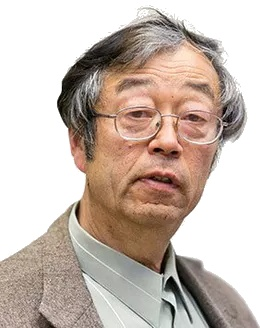
\includegraphics[width=0.5cm]{satoshi.jpg}};
\node             [opacity=0.7] at (program-icon |- mine) {
\includegraphics[width=0.5cm]{worldwide.png}};

\node (proposals-icon) at (mine-icon |- proposals) {
\includegraphics[width=0.5cm]{worldwide.png}};

\draw [Arrow] (whitepaper) -- (program);
\draw [Arrow] (program) -- (mine);
\draw [Arrow] (mine) -- (proposals);

\node (centralized) [right=of whitepaper.north east, anchor=south west, xshift=-0.5cm] {\color{DarkViolet} centralized};
\node (decentralized) [anchor=north] at (centralized |- proposals.south) {\color{DeepSkyBlue} decentralized};
\path[shade, top color=DarkViolet, bottom color=DeepSkyBlue] ([xshift=-0.1cm]centralized.south) rectangle ([xshift=0.1cm]decentralized.north);
\end{tikzpicture}
\end{figure}
\end{onlyenv}

\item<3-> A DApp can be a protocol or a group of smart contracts.
\item<4-> In this project we mainly grapple one or a couple of smart contracts, and we do not zero in the decentralization part.
\end{itemize}

\end{frame}


\begin{frame}[t]{RM2PT}
\etal{Yang}~[5] proposed RM2PT to transform a requirement document into a Java desktop program.
\onslide*<2>{
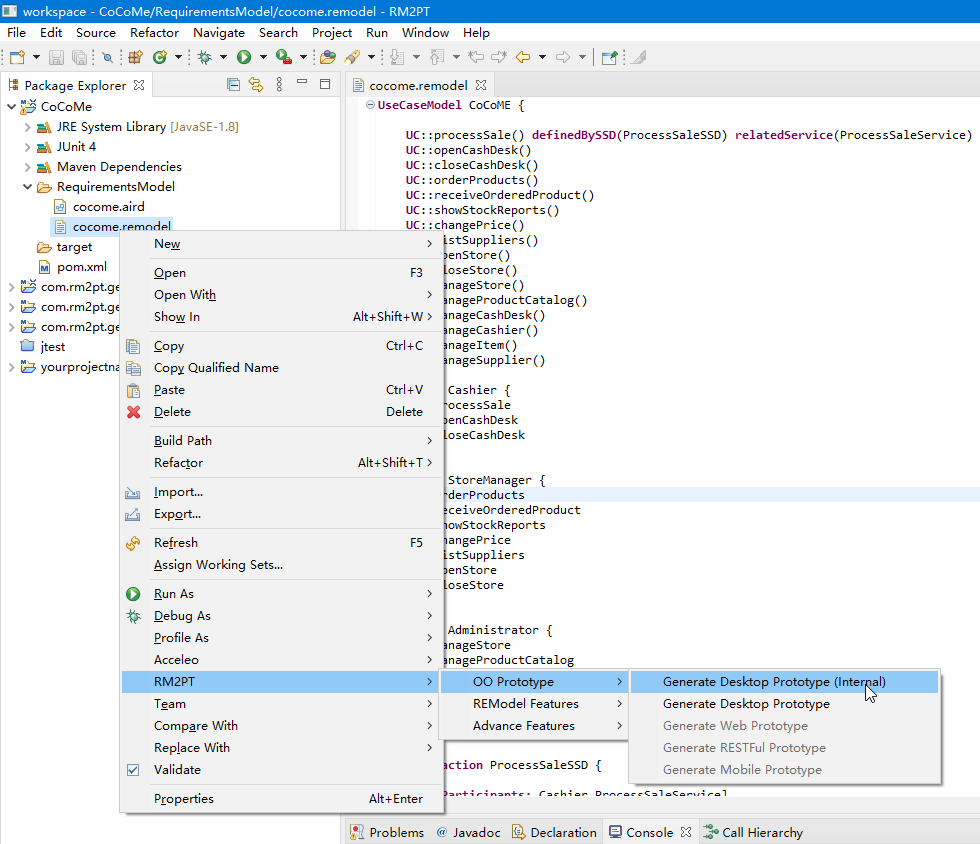
\includegraphics[width=0.7\linewidth]{RM2PT-generate}
}
\onslide*<3>{
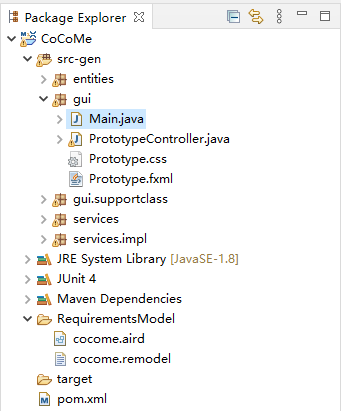
\includegraphics[width=0.5\linewidth]{rm2pt-folder-structure.png}
}
\onslide*<4>{
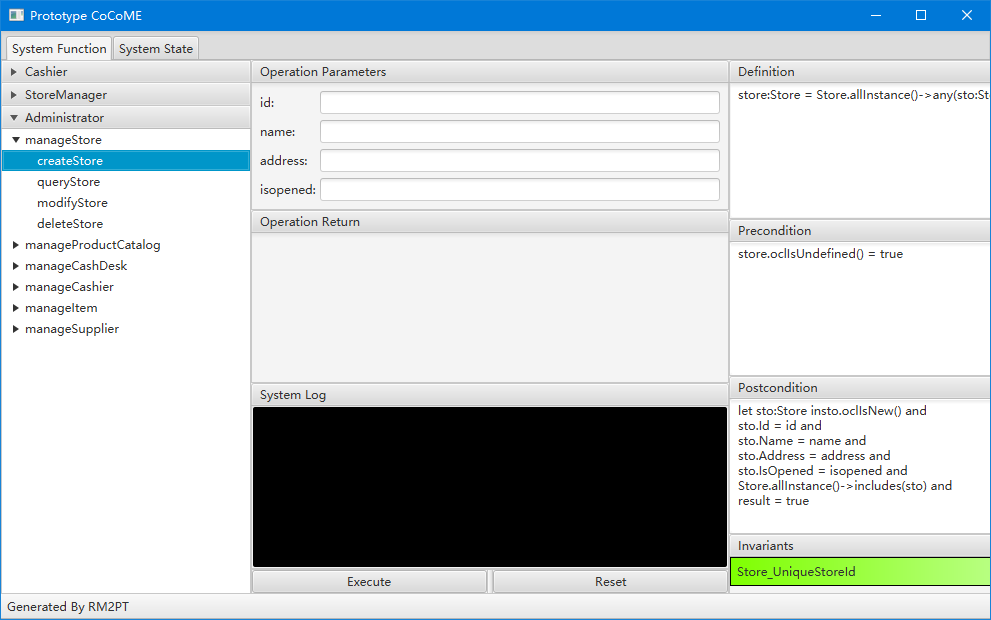
\includegraphics[width=\linewidth]{cocome-javafx.png}
}

\onslide<5>{
We contemplate to improve RM2PT so that it can generate smart contracts.
}

\end{frame}

\section{Literature Review}
\begin{frame}{Source Code Classification}

\begin{itemize}
\item \etal{Allamanis}~[6] proposed the naturalness hypothesis.
\begin{itemize}
\item Programming languages are like natural languages to a great extent.
\end{itemize}

\item  More and more work in software engineering start to use neural networks.
\begin{itemize}
\item neural machine translation (NMT), transformers
\end{itemize}
\end{itemize}
\end{frame}

\begin{frame}{Neural Networks in Source Code Classification}


\begin{itemize}
\item  Grammformers~[7] takes the context text and generates next code statements. The generated statements may contain holes.

\item \etal{Alexandru}~[12] used NMT to annotate source code tokens with typing.

\item \textsc{JSNice}~[13] predicts names of JavaScript identifiers and type annotations of variables.

\item \etal{Mou}~[14] used a convolutional neural network to classify programs by functionalities.

\item detection of variable misuse~[9],
bug localization~[10],
API suggestion~[11],
code completion~[15]
\end{itemize}
\end{frame}

\begin{frame}{Datasets for Source Code Classification}
\begin{itemize}
\item \etal{Jiang}~[8] collected a dataset of \num{1006} repositories from GitHub.
\begin{itemize}
\item unlabeled
\item mixed with Java and other languages
\end{itemize}

\item The dataset created by the authors of RMiner~[16] comprises \num{3188} refactorings found in 538 commits from 185 projects.
\begin{itemize}
\item allow functional changes
\end{itemize}
\end{itemize}

\end{frame}



\begin{frame}{Smart Contracts~[18]}

\begin{figure}
\centering
\begin{subfigure}[T]{0.3\textwidth}
	\includegraphics[width=\textwidth]{"smart contract architecture"}
	\caption{smart contract architecture model}
\end{subfigure}
\hfill
\begin{subfigure}[T]{0.65\textwidth}
	\includegraphics[width=\textwidth]{smart contract states.pdf}
	\caption{Finite-state of smart contract}
\end{subfigure}
\end{figure}


\end{frame}


%\begin{frame}{Duplicated Computing}
%\begin{itemize}
%\item Shae and Tsai~[] argue smart contracts are duplicated computing rather than distributed computing.
%\item<2-> They proposed a blockchain architecture for precision medicine.
%\begin{itemize}
%\item Smart contracts execute on chain.
%\item Applications run on a personal computer and call smart contracts
%\item Miners run the smart contract. The smart contract can be a Tensorflow program.
%\end{itemize}
%\end{itemize}
%\end{frame}

\begin{frame}{Distinctions between smart contract and OO languages}

\begin{itemize}
\item Reentrancy
	\begin{itemize}
	\item Smart contracts tend to call each other.
	\item The local states of one smart contract can only be modified by its own code.
	\end{itemize}

\item No multi-threading despite of attempts~[28,29]

\item \etal{Bram}~[20] holds that access control restrictions are a necessary part of the public specification of a contract.
\begin{itemize}
\item invented a DSL for Ethereum smart contract verification
\item not use Object Constraint Language (OCL)
\end{itemize}
\end{itemize}
\end{frame}


\begin{frame}{Transformation}

\begin{itemize}
\item State-of-the-art research is able to turn UML into mostly executable code~[22], including RM2PT.
\item RM2PT is able to complete 93.65\% of system operations.
\begin{itemize}
\item can check pre-conditions, post-conditions, and invariants
\item a runtime validation approach
\item<2-> These condition checking statements are transformed from OCL.
\item<3-> The language of the requirement document as a whole is unspecified.
\end{itemize}

\end{itemize}

\end{frame}

\begin{frame}{Verifying Smart Contract}
\onslide<+->
\begin{itemize}
\item Runtime Checking
\begin{itemize}
%\item<+-> RM2PT uses this approach.
\item<+-> ContractLarva~[23] uses Dynamic Automata with Timers and Events. It allows users to supply pre- and post-conditions for Ethereum.
\item<+-> Solythesis~[24] supports quantifiers, e.g., ``for all'', ``exists''. \onslide<+->{It invented delta update and delta check techniques so it doesn't have to suffix the checking statements to every transaction.}
\end{itemize}
\item[]<+-> 
\includegraphics[width=0.8em]{check.png}  gain correctness or security guarantees
\item[]<.-> 
\includegraphics[width=0.8em]{cross.png} no longer Turing-complete


\item Static Analysis \onslide<+->{is hard.}
\begin{itemize}

\item<+-> formalize the requirements to a specification
\item<.-> abstract implementation to a formal mathematical model
\item<.-> check the model against the specification~[25]
\item<+-> Securify~[26] translates Solidity smart contract into Datalog and verifies security properties with a SMT solver.

\end{itemize}

\end{itemize}

\end{frame}


\begin{frame}[t]{Consensus Algorithm}
\begin{itemize}
\item The execution result of a smart contract must be in consensus to be added to the blockchain.

\onslide*<1>{
\begin{tikzpicture}[node distance=0.5cm and 1cm, scale=0.9, transform shape]
\node (application) [Process] {application layer};
\node (execution) [Process, below=of application] {execution layer};
\node (verification) [Process, below=of execution] {verification layer};
\node (sm) [Process, below=of verification] {smart contract layer};
\node (transmission) [Process, below=of sm] {transmission layer};
\node (data) [Process, below=of transmission] {data layer};

\draw [Arrow] (application) -- (execution);
\draw [Arrow] (execution) -- (verification);
\draw [Arrow] (verification) -- (sm);
\draw [Arrow] (sm) --  (transmission);
\draw [Arrow] (transmission) -- (data);

\path[draw=red] (verification) circle [x radius=2cm, y radius=0.7cm];
\end{tikzpicture}
}

\begin{itemize}
\item<2-> Poof of Work, Poof of Stake, Practical Byzantine Fault Tolerance
\item<2-> A group of miners run the same piece of code to check if they got the same result.
\item<3-> Shae and Tsai~[19] call it duplicated computing.
\end{itemize}

\item<4-> {[27]}~used communicating sequential processes and queuing theory to model the behavior of a consensus algorithm.
\end{itemize}

\end{frame}

\begin{frame}{Consensus Algorithm Example}
\begin{tikzpicture}[scale=0.8, transform shape]
\node (100) [Process] {block 100};
\node (101) [Process, right=of 100] {block 101};

\draw [Arrow] (100) -- ++(-2,0);
\draw [Arrow] (101) -- (100);

\node (m1) [below=1.2cm of 101.west] {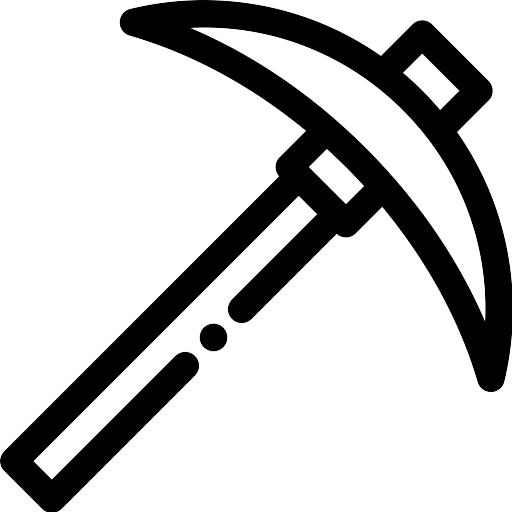
\includegraphics[width=1.5em]{miner.png}};
\node (m2) [below=0.5cm of m1] {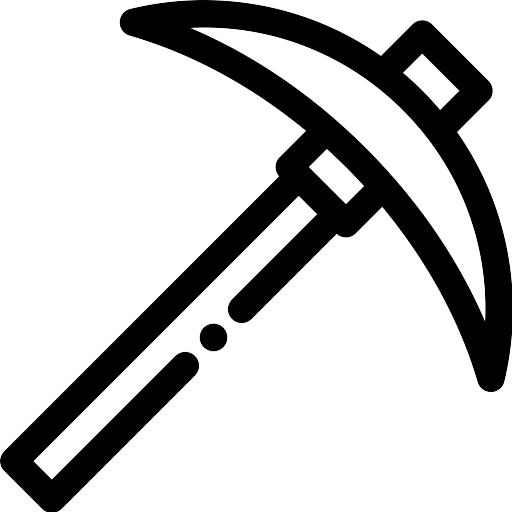
\includegraphics[width=1.5em]{miner.png}};
\node (m3) [below=0.5cm of m2] {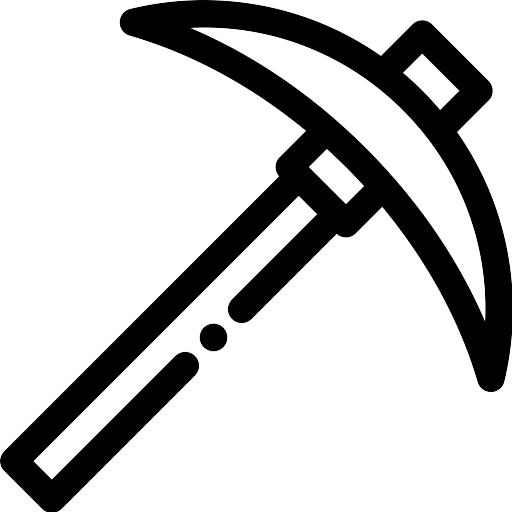
\includegraphics[width=1.5em]{miner.png}};

\onslide<2->{
\node [below=0.1cm of 101] { transaction proposal: \texttt{createStore(21,"Whole Foods")}};
}

\onslide<3-5>{
\node (r11) [right=0.1cm of m1] { \texttt{\{id:23, name:"Target"\}}};
\node (r12) [right=0.1cm of m2] { \texttt{\{id:22, name:"Ralphs"\}}};
\node (r13) [right=0.1cm of m3] { \texttt{\{id:24, name:"Bestbuy"\}}};
}
\onslide<4>{
\draw [draw=VioletRed, line width=0.1em] (r11.north west) rectangle (r13.south east);
\node [below=0.2cm of r13] {proposal responses};
}

\onslide<5>{
\node (sum1) [right=of r12, inner sep=0.1cm] {\color{red}{Not in consensus}};
\draw (r11.north east) -- ([xshift=1em]sum1.north west);
\draw (r13.south east) -- ([xshift=1em]sum1.south west);
}
\onslide<6->{
\node (r21) [right=0.1cm of m1] { \texttt{\{id:21, name:"Whole Foods"\}}};
\node (r22) [right=0.1cm of m2] { \texttt{\{id:21, name:"Whole Foods"\}}};
\node (r23) [right=0.1cm of m3] { \texttt{\{id:21, name:"Whole Foods"\}}};
}
\onslide<7->{
\node (sum2) [right=of r22, inner sep=0.1cm] {\color{Green}{In consensus}};
\draw (r21.north east) -- ([xshift=1em]sum2.north west);
\draw (r23.south east) -- ([xshift=1em]sum2.south west);
}
\onslide<8->{
\node (102) [Process, right=of 101] {block 102};
\draw [Arrow] (102) -- (101);
}
\end{tikzpicture}
	
\end{frame}

\begin{frame}{Smart Contract Applications}
\begin{itemize}
\item CoCoME~[30] describes a trading system in a supermarket setting.
	\begin{itemize}
	\item a local, single-user system, no parallelism
	\item RM2PT is fully tested on CoCoME.
	\end{itemize}

\item SLEX-Web~[31] is a web application for school.
\item Dao~[32] implemented a Vietnamese certificates application called ECefblock running on Hyperledger Fabric.
	\begin{itemize}
	\item in MVC pattern
	\item has requirement documents
	\end{itemize}
\end{itemize}
\end{frame}

\section{Problem Formulation}

\begin{frame}{Tech Stack of Smart Contracts}
\onslide*<1>{
\begin{figure}
\centering
\includegraphics[width=\linewidth]{techstack}
\end{figure}
}

\onslide*<2->{
\begin{itemize}
\item Hyperledger Fabric
\item Java
\item on-chain
\item pBFT
\item 3200 tx/s in HF 1.2*
\end{itemize}

* FastFabric: Scaling Hyperledger Fabric to 20,000 Transactions per Second
}


\end{frame}


\begin{frame}{Aims and Objectives}

Identification\\
\begin{enumerate}
\item study characteristics of blockchains and smart contracts
\item find out which functional implementations are transformable
%in MVC, no multi-threading
\item train classification neural networks to identify these patterns
\end{enumerate}

Transformation\\
\begin{enumerate}
\item transform source code to HyperLedger Java
\item add static analysis or runtime checking
\item find a model to formally describe the smart contract
\end{enumerate}

\end{frame}

\begin{frame}{Relevance, Novelty and Originality}
\begin{itemize}
\item The use of neural network in program analysis is lacking.
\item The transformation rules encoded in RM2PT are manually devised without much theory support.
\item I will use neural network.
\begin{itemize}
\item no need for a rigid syntax parser
\item Neural network delivers a percentage.
\item extend RM2PT to generate smart contract applications
\end{itemize}
\end{itemize}


\end{frame}

\section{Methodology}
\begin{frame}[t]
\frametitle{\onslide<2->{Properties of Smart Contracts}}
\begin{itemize}
\item<2-> literature review
	\begin{itemize}
	\item differences between smart contracts and DApp~[3]
	\item duplicated computing~[19]
	\item smart contract architecture model and finite-state machine~[18]
	\end{itemize}

\item<3-> pick up theories of programming languages in order to find a mathematical model, suggested by~[25]

\onslide*<4>{
\begin{figure}
\centering
\begin{subfigure}{0.25\textwidth}
	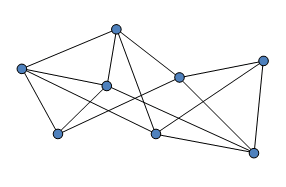
\includegraphics[width=\textwidth]{graph_theory.png}
\end{subfigure}
\hfill
\begin{subfigure}{0.25\textwidth}
	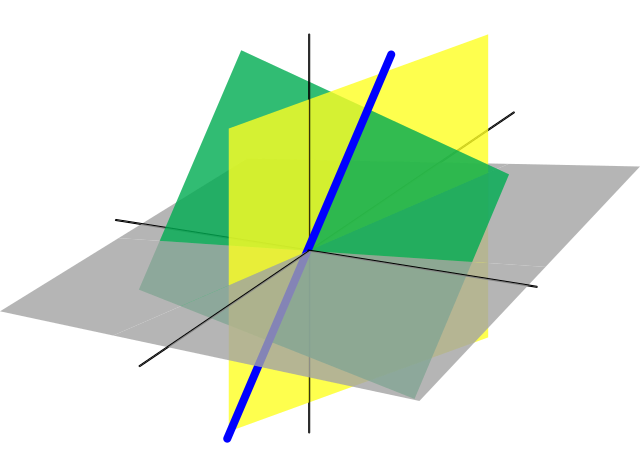
\includegraphics[width=\textwidth]{linear-algebra.png}
\end{subfigure}
\hfill
\begin{subfigure}{0.25\textwidth}
	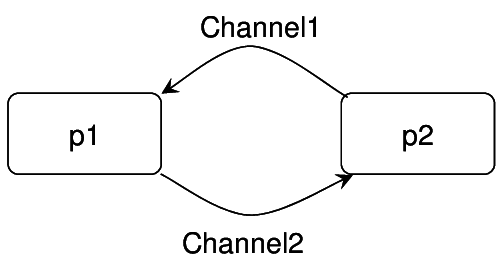
\includegraphics[width=\textwidth]{csp.png}
\end{subfigure}
\end{figure}
}


\item<5-> investigate theoretical differences between smart contract and traditional local programs
	\begin{itemize}
	\item check parallel properties and data persistence
	\end{itemize}
\item<6-> Finally, publish papers on the theory section of smart contracts
\end{itemize}
\end{frame}


\begin{frame}[t]{Identification of Functional Implementation}
\begin{itemize}
\item I have already looked into using neural networks to analyze program source code.
	\begin{itemize}
	\item Q.~Gu and W.~Ke, ``A neural architecture for detecting identifier renaming from diff,'' in {\em International Conference on Intelligent Data Engineering and Automated Learning}, pp.~33--44, Springer, 2021.~
\includegraphics[height=2ex, angle=20,origin=c, ]{favourite.png}
	\end{itemize}

\item train a neural network to automatically filter the conventional programs for the next transformation
\onslide*<+>{
\begin{figure}
\centering
\begin{subfigure}{0.20\textwidth}
	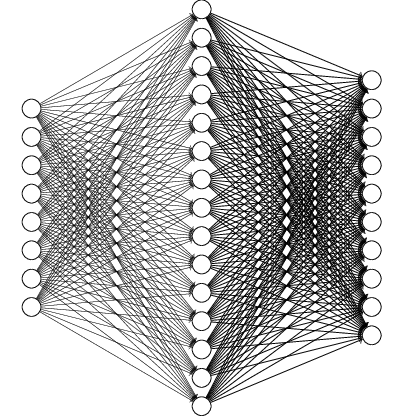
\includegraphics[width=\textwidth]{dense-layers.png}
\end{subfigure}
\hfill
\begin{subfigure}{0.20\textwidth}
	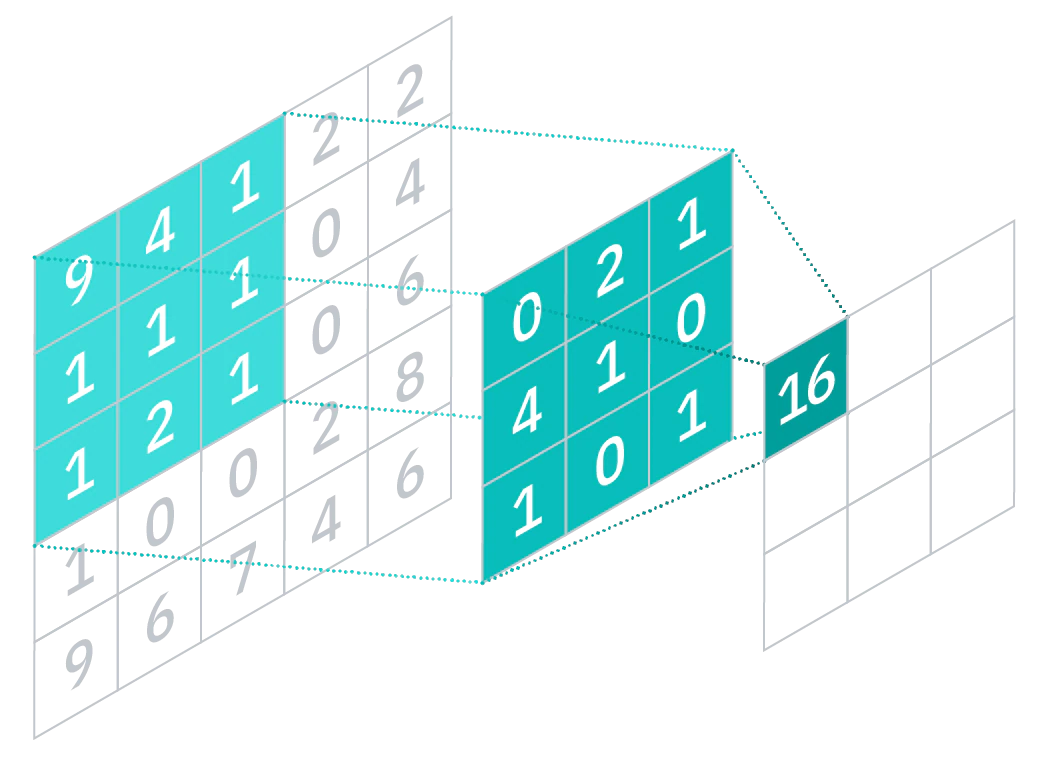
\includegraphics[width=\textwidth]{cnn.png}
\end{subfigure}
\hfill
\begin{subfigure}{0.20\textwidth}
	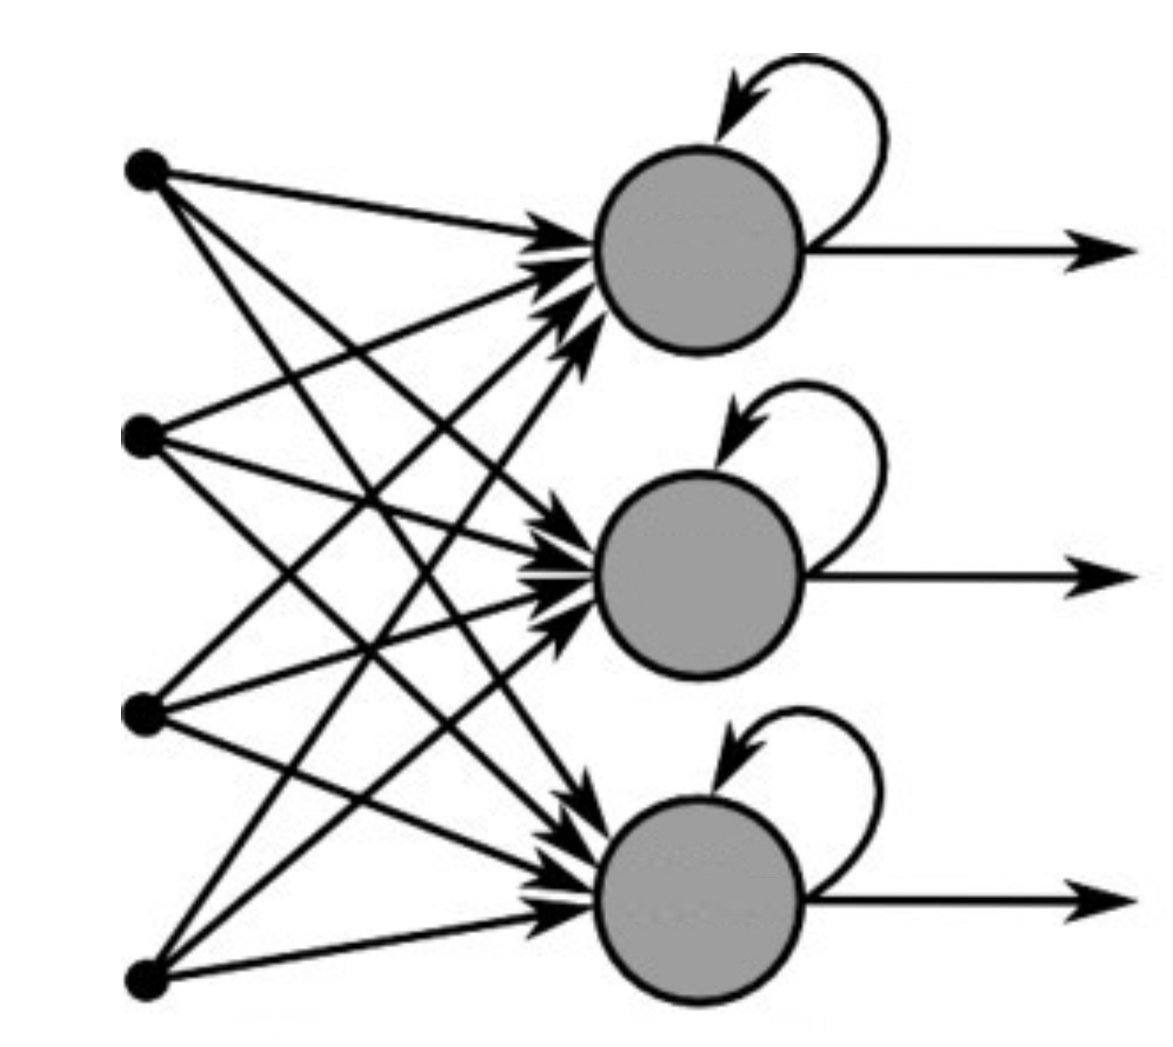
\includegraphics[width=\textwidth]{rnn.png}
\end{subfigure}
\hfill
\begin{subfigure}{0.20\textwidth}
	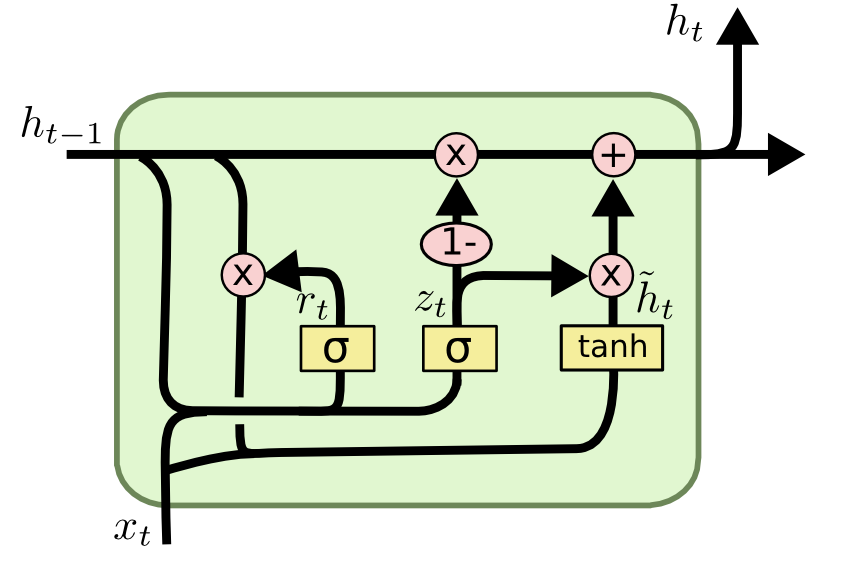
\includegraphics[width=\textwidth]{lstm.png}
\end{subfigure}
\end{figure}
}
\end{itemize}

\end{frame}


\begin{frame}{Transformation to Smart Contracts}
\tikzstyle{Text} = [text centered, align=center]
\tikzset{Link/.style={thick, ->, >=stealth, dashed, blue}}

\centering
\begin{tikzpicture}[scale=0.8, transform shape, node distance=0.8cm and 1cm]
\node (RM2Hyperledger) [Process] {RM2Hyperledger};
\node (cases) [Process,below=of RM2Hyperledger.south] {Study cases};
\node (data)  [Process,below=of cases.south]{Data persistence};
\node (challenge) [Process,below=of data.south] {Challenge: post-conditions};
\node (evaluate) [Process,below=of challenge.south] {evaluate};

\draw [Arrow] (RM2Hyperledger) -- (cases);
\draw [Arrow] (cases) -- (data);
\draw [Arrow] (data) -- (challenge);
\draw [Arrow] (challenge) -- (evaluate);

\onslide<2>{
\node (1) [Text, right=2cm of RM2Hyperledger.east] {initially use rule-based transformation,\\then attempt neural networks};
\draw [Link] (RM2Hyperledger.east) -- (1.west);
}

\onslide<3>{
\node (2) [Text, right=2.5cm of cases.east] {CoCoME};
\node (3) [Text, below=of 2.south west, anchor=west] {SLEX-Web and ECefblock};
\draw [Link] (cases.east) -- (2.west);
\draw [Link] (cases.east) -- (3.west);
}

\onslide<4>{
\node (4) [Text, right=1.3cm of RM2Hyperledger.east, anchor=west] {One object must hold an unique identifier (PK)\\of another object\\and load the object from the chain\\when needed through the PK.};
\node (5) [Text, below=of 4.south west, anchor=west ] {on-chain};
\node (6) [Text, below=of 5.south west, anchor=west] {add or locate PK of each entity,\\add serialization support};
\node (7) [Text, below=of 6.south west, anchor=north west] {potentially invent a library\\for saving and loading data,\\like Object–relational mapping};
\draw [Link] (data.east) -- (4.west);
\draw [Link] (data.east) -- (5.west);
\draw [Link] (data.east) -- (6.west);
\draw [Link] (data.east) -- (7.west);
}

\onslide<5>{
\node (8) [Text, right=1cm of challenge.east, anchor=west] {results are not yet committed};
\node (9) [Text, below=of 8.south west, anchor=north west] {a second smart contract, \\checking program local states, \\custom consensus algorithm, \\lazy evaluation};
\draw [Link] (challenge.east) -- (8.west);
\draw [Link] (challenge.east) -- (9.west);
}
\end{tikzpicture}

\end{frame}


\begin{frame}{Verification of Smart Contracts}
\begin{itemize}
\item RM2PT adds invariants, pre- and post-conditions to all operations, a powerful approach.
	\begin{itemize}
	\item inter-smart contract reentrancy does not corrupt the memory
	\item has large runtime overhead for smart contracts~[24]
	\end{itemize}

\item<2-> Nevertheless, I will follow RM2PT and perform runtime validation.

\item<3-> use a formal mathematical model to prove the properties of smart contract
	\begin{itemize}
	\item A SMT solver may be used.
	\end{itemize}
\end{itemize}

\end{frame}

\section{Schedules and Milestones}

\begin{frame}{Schedules}


\tikzstyle{Text} = [text centered, align=center]
\tikzset{Link/.style={line width=0.1cm, ->, >=stealth, dashed, blue}}
\centering
\begin{tikzpicture}[xscale=0.4, yscale=0.3, transform shape]

\node[single arrow,top color=Red, bottom color=Green, minimum height=25cm, rotate=-90,  inner sep=0.3cm]  at (0,-12.5) {};

%\node at (-1, 0) {May 2021};
%\node at (-1,-25) {June 2023};

\onslide<2->
\node [anchor=east] at (-1,-2) {\huge July 2021};
\node [anchor=west] at (2, -2) {\Huge I've submitted a paper on diff classification. 
\includegraphics[height=2ex, angle=20,origin=c, ]{favourite.png}};
\draw [Link] (2, -2) -- (0,-2);

\onslide<3->
\node [anchor=east] at (-1,-10) {\huge March 2022};
\node [anchor=west, Text] at (2,-10) {\Huge I'm working on smart contract generation\\\Huge and going to write a paper.};
\draw [Link] (2,-10) -- (0,-10);

\onslide<4->
\node [anchor=east] at (-1,-19) {\huge December 2022};
\node [anchor=west,Text] at (2,-19) {\Huge I will work on the theory part of smart contract.\\\Huge The paper may focus on refinement calculus\\\Huge  and use pre-order or partial order in proofs.};
\draw [Link] (2,-19) -- (0,-19);


\onslide<5->
\node [anchor=east] at (-1,-23) {\huge April 2023};
\node [anchor=west,Text] at (2,-23) {\Huge I shall commence writing my doctoral thesis.};
\draw [Link] (2,-23) -- (0,-23);

\end{tikzpicture}

\end{frame}

\begin{frame}{Key milestones}
Conference list:\\
\begin{enumerate}
\item International Conference on Intelligent Data Engineering and Automated Learning (IDEAL)
\item IEEE/ACM International Conference on Automated Software Engineering (ASE)
\item IEEE DAPPS: \url{https://ieeedapps.net/}
\end{enumerate}

Journal list:\\
\begin{enumerate}
\item Frontiers of Computer Science
\item IEEE Transactions on Industrial Informatics
\item IEEE Transactions on Reliability
\end{enumerate}
\end{frame}

\begin{frame}{Potential publications}
\begin{description}
\item[Paper] RM2Hyperledger: Automated Prototype Generation From Requirements Model to Hyperledger Smart Contract
\item[Journal] Refining Conventional Applications to Smart Contracts
\item[Paper] A Neural Architecture for Classifying Refactoring Types from Diff
\item[Doctoral Thesis] Identification of Functional Implementation in Conventional Applications and Transformation to Smart Contracts
\end{description}
\end{frame}

\section{Conclusions}
\begin{frame}{Conclusions}

\begin{itemize}
\item Businesses and organizations are motivated to use smart contracts in their daily operations,
\begin{itemize}
\item but coding smart contracts is a big barrier for developers.
\end{itemize}

\item An opportunity to automatically transform conventional functional implementations to smart contracts
\begin{itemize}
\item Such transformation is not 100\%  complete.
\end{itemize}

\item use a neural network to identify the application
\begin{itemize}
\item a paper published 
\includegraphics[height=2ex, angle=20,origin=c, ]{favourite.png}
\end{itemize}

\item use CoCoME as my first study case
\item prove soundness of the transformation
\end{itemize}


\end{frame}


\begin{frame}[t]{References}
See the paper
\end{frame}


{
	\usebackgroundtemplate{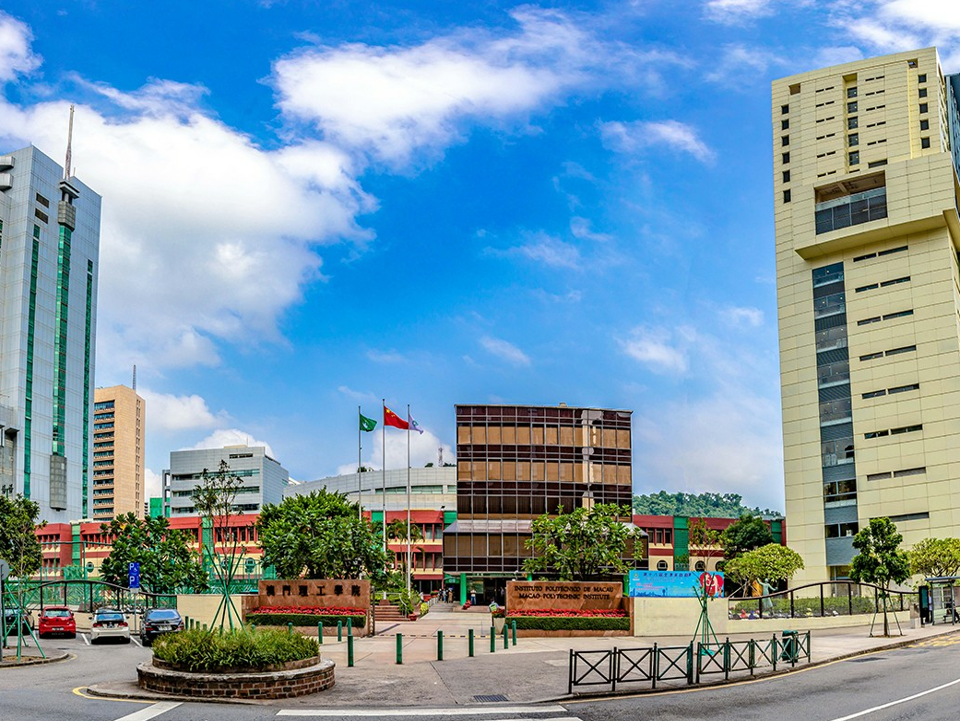
\includegraphics[height=\paperheight]{MPI-front-gate.png}}%
	\contourlength{.06em}
	\begin{frame}[plain]
	\begin{tikzpicture}[overlay, remember picture]
	\node[yshift=1cm] at (current page.center) {\contour{white}{\Huge Thank you!}};
	\end{tikzpicture}
	\end{frame}
}

\end{document}
